\documentclass{article}
\usepackage{ketpic,ketlayer}
\usepackage{amsmath,amssymb}
\usepackage{graphicx}
\usepackage{xcolor}
\usepackage{bm,enumerate}
\usepackage[colorlinks=true,urlcolor=blue]{hyperref}

\setmargin{20}{15}{15}{15}

\renewcommand{\labelitemi}{$\cdot$}

\pagestyle{empty}

\begin{document}

\begin{center}
Installing of KeTCindy 
\end{center}

\hfill Modified\ :\ \today

\begin{enumerate}[\bf\large 1.]
\item Install Cinderella, R, Maxima (and Sumatra only for Windows)
 \begin{itemize}
 \item \url{https://beta.cinderella.de}  (Cinderella)
 \item \url{https://cran.r-project.org}   (R)
 \item \url{https://sourceforge.net/projects/maxima/files}  (Maxima)
 \item \url{https://www.sumatrapdfreader.org/download-free-pdf-viewer.html} (Sumatra)\\
\hspace*{5mm}Rem) Sumatra should be installed in Program Files (or x86).
 \end{itemize}
\item Install a TeX system if no one has been installed.
 \begin{enumerate}[(1)]
 \item TeXLive is recommended.
    \begin{itemize}
    \item KeTCindy has been implemented (2018 or later).
    \end{itemize}
 \item KeTTeX is a light-weighted TeXLive.
    \begin{itemize}
    \item It is downloadable from\\
    \hspace*{5mm}Mac (kettex.dmg)\\
    \hspace*{10mm}\url{https://www.dropbox.com/s/dc4inuk06t07g26/kettex.dmg?dl=0}\\
    \hspace*{5mm}Windows (kettex.exe)\\
    \hspace*{10mm}\url{https://www.dropbox.com/s/fthw4btjqqs33tc/kettex.exe?dl=0}\\
    \hspace*{5mm}Linux (kettex.tar.xz)\\
    \hspace*{10mm}\url{https://www.dropbox.com/s/vg8p07832e9hzlk/KeTTeX-linux-20171022.tar.xz?dl=0}
     \item Move unzipped kettex into the folder /Applications for Mac and C:\textbackslash\ for Windows.
    \end{itemize}
 \end{enumerate}

\item Install KeTCindy
  \begin{enumerate}[(1)]
  \item Download ketcindy from CTAN(\url{https://ctan.org}).\\
  \hspace*{10mm}Search ketcindy $>$ Pack­age ketcindy $>$ Download\ \ ('ketcindy')
    \begin{itemize}
    \item[Rem)]The latest version is downloadable from Repository:\\
         \hspace*{5mm}Clone or download $>$ Download ZIP\ \ ('ketcindy-master')
    \end{itemize}
  \item Double click \verb|ketcindysettings.cdy| in the folder.
    \begin{itemize}
    \item Set Cinderella as the executive program if necessary.
    \item Reboot Cinderella if other cdy files are open.
   \end{itemize}

\vspace{2mm}

\begin{layer}{140}{0}
\putnotese{27}{20}{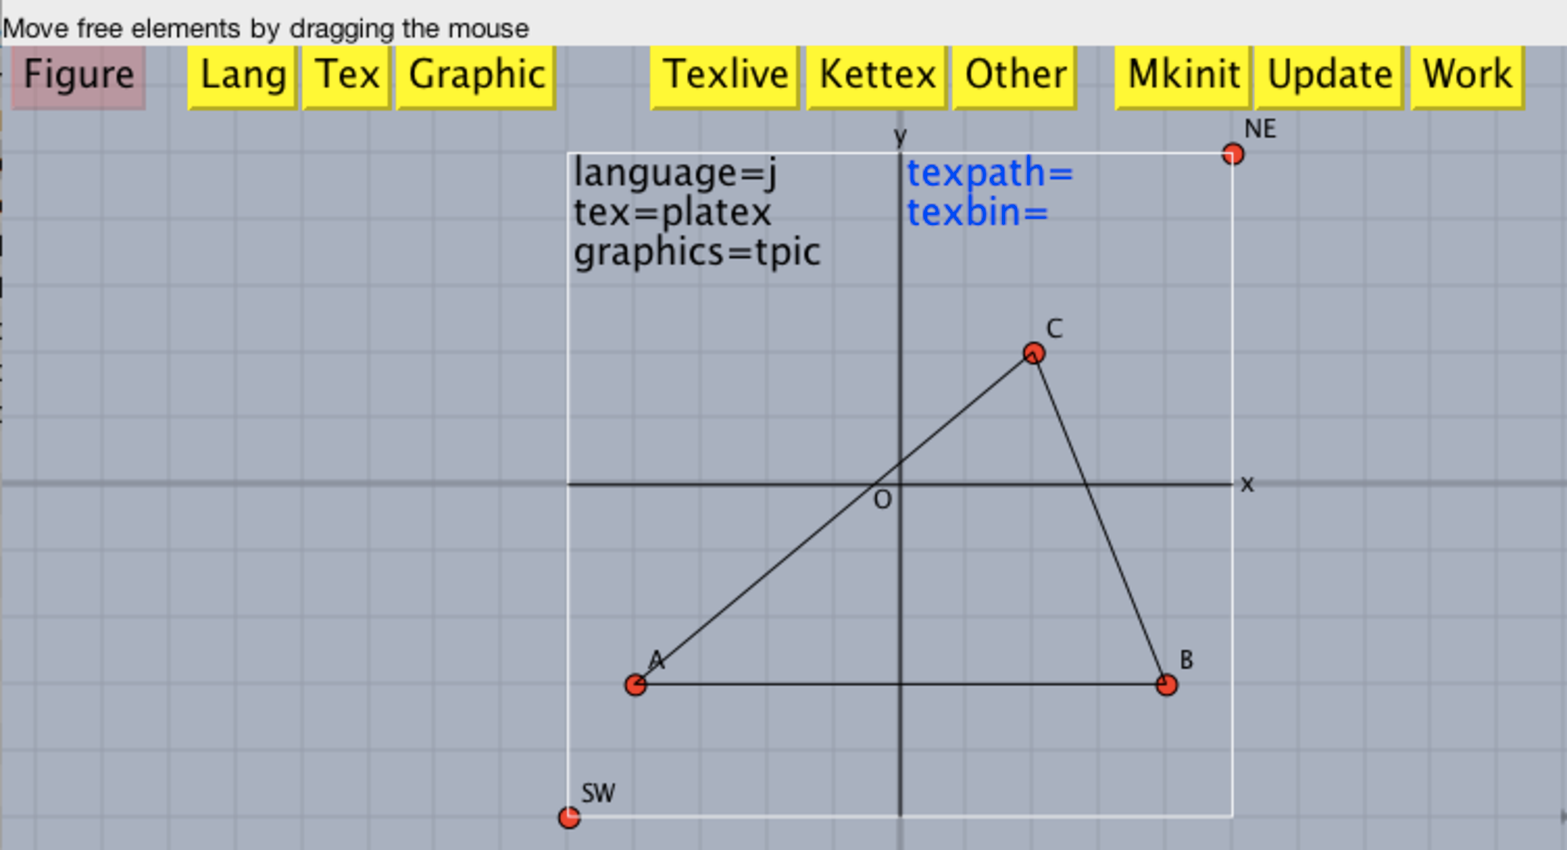
\includegraphics[bb=0.00 0.00 752.00 408.00,width=100mm]{Fig/setting.pdf}}
\putnotee{0}{5}{\bf [1]\ Select language,etc}
\putnotese{3}{10}{\underline{Language}}
\putnotese{7}{15}{Japanese, English}
\putnotese{3}{20}{\underline{\TeX}}
\putnotese{5}{24}{\begin{tabular}{l}
platex\\uplatex\\latex\\xelatex\\pdflatex\\lualatex\end{tabular}}
\putnotese{3}{51}{\underline{Graphic Code}}
\putnotese{5}{55}{\begin{tabular}{l}tpic\\pict2e\\tikz\end{tabular}}
\arrowline{47}{20}{17}{135}
\putnoten{83}{7}{\bf [2]Select \TeX\ sytem}
\arrowline{83}{20}{13}{90}
\putnotee{125}{5}{\bf [3]\ Folder operation}
\arrowline{110}{20}{20}{45}
\putnotese{131}{10}{\underline{Mkinit}}
\putnotese{133}{15}{\begin{minipage}[t]{36mm}%
Create initialization file 'ketcindy.ini' in user's home.
\end{minipage}}
\putnotese{131}{29}{\underline{Update}}
\putnotese{133}{34.5}{Update ketcindy in \TeX}
\putnotese{133}{39.5}{$\cdot$ if error occurs,}%
\putnotese{137}{44.5}{1) Open 'update'}%
\putnotese{137}{49.5}{2) Execute shell file}%
\putnotese{137}{54.5}{3) For Windows, run}%
\putnotese{139}{59.5}{as an administrator}%
\putnotese{139}{65}{with right-click.}
\putnotese{131}{70}{\underline{Work}}
\putnotese{133}{75}{\begin{minipage}[t]{36mm}%
Create folder 'ketcindy' in user's home.\\
Manuals, samples will be copied.
\end{minipage}}
\end{layer}

\vspace{75mm}

{\bf [4]\ Test run}\\
\hspace*{10mm}The figure may not appear at first.\\
\hspace*{10mm}Press \verb|Figure| button, and the pdf will be displayed.

  \end{enumerate}

  \end{enumerate}

\end{document}